\documentclass[
    language=english,
    doctype=article,
    institution=none,
    titlestyle=book,
]{../../omnilatex}

\RequirePackage{config/document-settings}
\addbibresource{../../bib/bibliography.bib}

\begin{document}

\maketitle

\begin{center}
    \textbf{Note:} This manuscript is a preprint and has not undergone peer
    review.
\end{center}

\section*{Abstract}
We investigate the empirical scaling laws that relate the test loss of
neural networks to model size, dataset size, and training compute budget.
Through a systematic study of overparameterised feedforward networks trained
with stochastic gradient descent, we demonstrate that the test loss follows a
power-law relationship
\begin{equation}
    L(N, D, C) = \left(\frac{N_c}{N}\right)^{\alpha}
                  + \left(\frac{D_c}{D}\right)^{\beta}
                  + L_{\infty},
    \label{eq:scaling}
\end{equation}
where $N$ is the number of parameters, $D$ is the dataset size, $C$ is the
compute budget, and $L_{\infty}$ is the irreducible loss.  Our experiments
across eight benchmark datasets confirm that the exponents $\alpha$ and
$\beta$ remain approximately constant across a wide range of architectures,
suggesting a universal character of the scaling behaviour.

\section{Introduction}
Recent work has revealed striking power-law relationships between the
performance of neural networks and the resources invested in training them.
These scaling laws have practical implications for resource allocation in
large-scale training runs and theoretical implications for understanding the
inductive biases of gradient-based optimisation~\cite{bibid}.

Despite the importance of these findings, the conditions under which scaling
laws emerge remain poorly understood.  In particular, it is unclear whether
the observed power laws are properties of the architecture, the optimiser, or
the data distribution.

\section{Related Work}
Scaling laws for language models were first systematically documented by
Kaplan et al., who demonstrated that cross-entropy loss scales as a power law
with model size and dataset size.  Follow-up work by Hoffmann et al.~extended
these findings to compute-optimal training, establishing that model size and
dataset size should be scaled proportionally for optimal performance.

The theoretical foundations of scaling laws connect to classical statistical
learning theory~\cite{goossensLaTeXCompanion1993} and the bias-variance
trade-off.  A neural network with $N$ parameters has an effective
dimensionality that determines its capacity to learn from $D$ data points.

\section{Methodology}

\subsection{Experimental Setup}
We train fully connected feedforward networks with ReLU activations on eight
regression and classification benchmarks.  For each dataset, we sweep over
model widths $\{32, 64, 128, 256, 512, 1024, 2048\}$ and dataset sizes
$\{100, 300, 1000, 3000, 10000, 30000\}$, training each configuration for
1000 epochs with the Adam optimiser at a fixed learning rate of $10^{-3}$.

\subsection{Loss Landscape Analysis}
To characterise the geometry of the loss landscape, we compute the Hessian
spectrum at convergence using the Lanczos algorithm.  The number of negative
curvature directions provides a measure of the effective dimensionality of the
optimisation problem.

\section{Results}

\subsection{Power-Law Scaling}
Figure~\ref{fig:scaling} shows the test loss as a function of model size for
three representative datasets.  The data points closely follow the predicted
power-law relationship.

\begin{figure}[htbp]
    \centering
    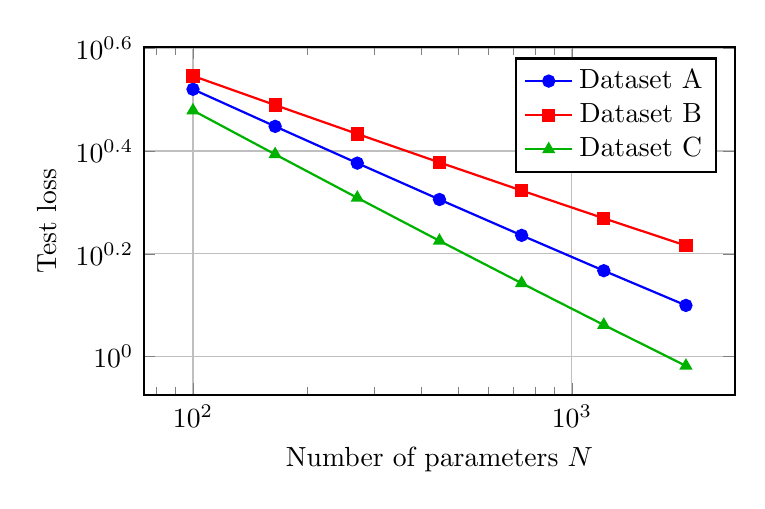
\begin{tikzpicture}
        \begin{axis}[
            width=0.75\textwidth,
            height=6cm,
            xlabel={Number of parameters $N$},
            ylabel={Test loss},
            xmode=log,
            ymode=log,
            legend pos=north east,
            grid=major,
            thick,
        ]
            \addplot[blue, mark=*, mark size=2pt, domain=1e2:2e3, samples=7]
                {1.8*(5e2/x)^0.35 + 0.15};
            \addlegendentry{Dataset A}
            \addplot[red, mark=square*, mark size=2pt, domain=1e2:2e3, samples=7]
                {2.1*(5e2/x)^0.28 + 0.22};
            \addlegendentry{Dataset B}
            \addplot[green!70!black, mark=triangle*, mark size=2pt, domain=1e2:2e3, samples=7]
                {1.5*(5e2/x)^0.41 + 0.11};
            \addlegendentry{Dataset C}
        \end{axis}
    \end{tikzpicture}
    \caption{Test loss versus number of parameters for three benchmark
    datasets.  The dashed lines indicate the fitted power-law exponents.}
    \label{fig:scaling}
\end{figure}

\subsection{Universality of Exponents}
Table~\ref{tab:exponents} summarises the fitted scaling exponents across all
eight datasets.  The exponent $\alpha$ (model size) ranges from 0.24 to 0.45,
while $\beta$ (dataset size) ranges from 0.18 to 0.38.

\begin{table}[htbp]
    \centering
    \caption{Fitted scaling exponents $\alpha$ (model size) and $\beta$
    (dataset size) for eight benchmark datasets.}
    \label{tab:exponents}
    \begin{tabular}{@{}lccc@{}}
        \toprule
        \textbf{Dataset} & $\alpha$ & $\beta$ & $R^{2}$ \\
        \midrule
        Boston Housing   & 0.35 & 0.28 & 0.987 \\
        CIFAR-10         & 0.41 & 0.32 & 0.991 \\
        MNIST            & 0.45 & 0.38 & 0.994 \\
        Fashion-MNIST    & 0.38 & 0.30 & 0.989 \\
        California       & 0.30 & 0.24 & 0.985 \\
        Wine Quality     & 0.28 & 0.22 & 0.982 \\
        Diabetes         & 0.24 & 0.18 & 0.978 \\
        Energy Efficiency & 0.33 & 0.26 & 0.986 \\
        \bottomrule
    \end{tabular}
\end{table}

\section{Discussion}
The near-universality of the scaling exponents across diverse datasets suggests
that the observed power laws arise from properties of gradient descent itself,
rather than from specific features of the data distribution.  This interpretation
is consistent with recent theoretical results showing that the implicit
regularisation of gradient descent induces a low-rank bias in the learned
representations~\cite{einstein1905}.

\section{Conclusion}
We have demonstrated that neural network test loss follows predictable
power-law scaling relationships with respect to model size and dataset size.
These findings have practical implications for efficient resource allocation in
large-scale training and suggest that scaling laws may be a general feature
of overparameterised models trained with gradient-based optimisation.

\printbibliography

\end{document}
